\chapter{Reference Tracking and Disturbance Rejection}

\section{Introduction}
\hl{Specific work done to extend the PILCO algorithm. Will essentially expand out the CDC paper but sell it as a more general method for incorporating known parts of system dynamics into the learning framework. Finally, include the results from the pendulum in simulation and hardware.}


\section{The LQG Trick}
In this section, the LQ approach to tracking control outlined in Chapter 3 of \cite{BGW90} is reviewed. Consider the reference tracking control of a stochastic, discrete-time, Linear Time-Invariant (LTI) system given by 
\begin{equation}
\bx_{k+1} = A\bx_k + B\bu_k + \mathbf{w}_k,
\end{equation}
with state, input and noise terms as defined in. 

\begin{figure}[] %%%
\centering
\tikzstyle{block} = [thick, rectangle, draw, text width=7em, text centered, rounded corners, minimum height=4em, fill=black!15]
\tikzstyle{bloc2k} = [thick,rectangle, draw, text width=9em, text centered, rounded corners, minimum height=4em, fill=black!25]
\tikzstyle{sum} = [thick,circle, draw, minimum height=.5cm]
\tikzstyle{line} = [draw, -latex']

\begin{tikzpicture}[rounded corners]
	
	% Place nodes
	\node at(0,0) [block](controller){\textbf{Policy} \\$\pi(\bx^{\text{tr}})$};
	\node at(5,0) [bloc2k](system){\textbf{System} \\$\bx'=f(\bx,\bu) + \mathbf{w}$};
	
	% Draw arrows
	\path[line] (controller.east) -- (system.west);
	\path[line] (system.east) -| (8,1.5) -| (-2.5,0.5) -- ([yshift=.5cm]controller.west);
	\path[line] (-2.5,-0.5) -- ([yshift=-.5cm]controller.west);
	
	
	% Labels
	\node at (2.3,.3) {$\bu$};
	\node at (-2,.8) {$\bx$};
	\node at (-2,-.15) {$\bx^{\mathbf{r}}$};
	\node at (7.5,.3) {$\bx$};

\end{tikzpicture}
\caption{Block diagram displaying a system controlled according to a policy $\pi(\cdot)$ which has access to future reference trajectory information $\bx^{\br}$. The term $z^{-1}$ indicates a one-step delay.}
\label{figs:lqsetup}
\end{figure} %%%

The LQ tracking problem is an extension to the LQR problem by penalising state deviations from some reference trajectory $\br_k$. The policy also has access to the values of the reference trajectory for $H^{\br}$ timesteps in the future $\bx^{\br}_k$, where $\bx^{\br}_k \in \RR^{nH^{\br}}$ contains the stacked future trajectory information $[\br_k^\top \dots \br_{k+H^{\br}-1}^\top]^\top$. The controller setup is depicted in Figure~\ref{figs:lqsetup}. The finite horizon cost function is defined as follows
\begin{align}
\nonumber V (H,\bx_0) 
&= \sum_{k=0}^{H-1} \EE_{\bx_k}\Big[ (\bx_k-\br_k)^\top Q (\bx_k-\br_k) + \bu_k^\top R \bu_k \Big] \\
&+ \EE_{\bx_H}\Big[(\bx_H-\br_H)^\top P_H (\bx_H-\br_H) \Big].
\end{align}
Recognising that $\br_k$ is externally prescribed and that the policy will have access to the values of the reference trajectory $H^{\br}$ steps into the future, an artificial state-space model may be defined as
\begin{equation}
\bx^{\br}_{k+1} = A^{\br}\bx^{\br}_k + B^{\br} \mathbf{n}_k, \quad
\br_k = C^{\br} \bx^{\br}_{k}   \label{eqn:refsys} 
\end{equation}
where $\mathbf{n}_k \sim \cN(0,\Sigma_{\mathbf{n}})$. In the following $\Sigma_{\mathbf{n}}$ shall be set to~1. If it is assumed that the reference trajectory is generated by the following white noise driven, linear filtering system
\begin{equation}
\br_{k+1} = A^{\text{f}}\br_k + B^{\text{f}} \mathbf{n}_k
\label{eqn:linfil}
\end{equation}
with specified initial condition $\br_0$, then the state-space matrices are given by the following
\begin{align}
\nonumber A^{\br} &= \begin{bmatrix} 
\quad\mathbf{0}_{nH^{\br}\times H^{\br}} & \begin{matrix} I_{(n-1)H^{\br}} \\
 \Big[\mathbf{0}_{H^{\br} \times (n-2)H^{\br}}\;\; A^{\text{f}}\Big] \end{matrix}
\end{bmatrix}, \\
\nonumber B^{\br} &= \begin{bmatrix} \mathbf{0}_{(n-1)H^{\br}\times H^{\br}}  \\ B^{\text{f}} \end{bmatrix} , \;
 C^{\br} = \Big[I_{H^{\br}} \;\; \mathbf{0}_{H^{\br}\times (n-1)H^{\br}}\Big] 
\end{align}
%%%%%%%%%%%%%%
where $\mathbf{0}_{p\times q}$ is the $p$ by $q$ matrix of zeros. This formulation can characterise a wide range of reference signals. Two examples are shown in Figure~\ref{figs:examplerefs} of second-order filtered white noise and exponentially decaying sinusoids of a given frequency. In the sinusoid example $B^{\text{f}}=0$ but randomness arises by allowing a distribution over starting state $\br_0$.

The tracking problem may now be recast as a standard LQR problem by defining an augmented state vector $\bx^{\tr} := [\bx^\top, \bx^{\br\top}]^\top \in \RR^{n(H^{\br}+1)}$ and associated state-space equation
\begin{equation}
\bx^{\tr}_{k+1} = \begin{bmatrix} A & 0 \\ 0 & A^{\br} \end{bmatrix} \bx^{\tr}_k +
\begin{bmatrix} B \\ 0\end{bmatrix} \bu_k +
\begin{bmatrix} I & 0 \\ 0 & B^{\br} \end{bmatrix} \begin{bmatrix}\mathbf{w}_k \\ \mathbf{n}_k \end{bmatrix}.
\end{equation}
This leads to $\bx_k - \br_k = \begin{bmatrix} I & -C^{\br} \end{bmatrix}\bx^{\tr}_k$ and therefore a finite horizon LQR problem with $Q^{\tr} := \begin{bmatrix} I & -C^{\br} \end{bmatrix}^\top Q \begin{bmatrix} I & -C^{\br} \end{bmatrix}$ and  $P_H^{\tr} := \begin{bmatrix} I & -C^{\br} \end{bmatrix}^\top P_H \begin{bmatrix} I & -C^{\br} \end{bmatrix}$. In general, this leads to a linear time-varying control law $K^{\tr}_{H-k-1}$ which is undesirable in practice. However, applying $K = K^{\tr}_{H-1}$ as a time-invariant control law yields the associated \textit{receding horizon} policy.







\begin{figure}[t] %%% 
\centering
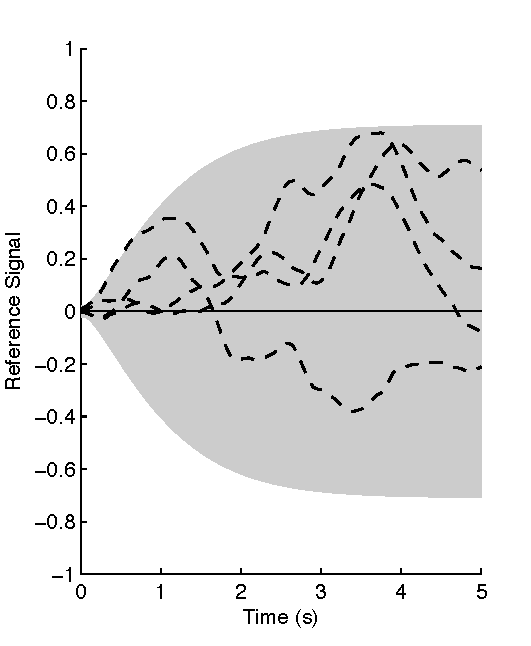
\includegraphics[scale=0.7, clip, trim = 0cm 0cm 0cm 0cm]{figs/refnoise.pdf}
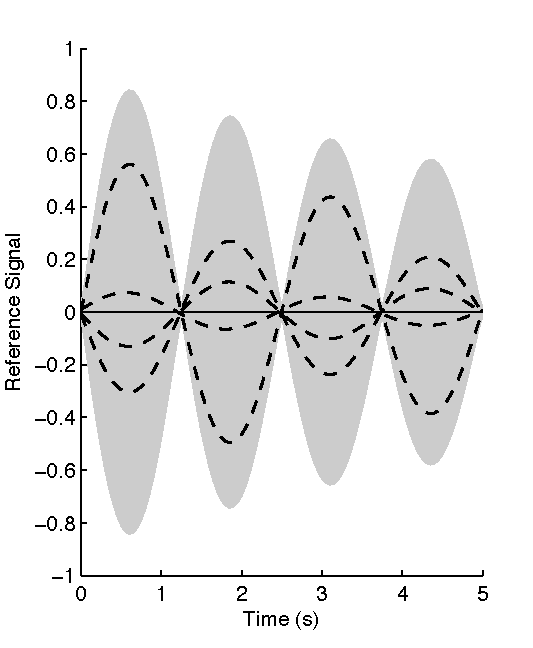
\includegraphics[scale=0.7, clip, trim = 0cm 0cm 0cm 0cm]{figs/refsine.pdf}
\caption{Illustration of the type of trajectories that can be modelled by the state space equation (\ref{eqn:linfil}). The left hand plot depicts second-order filtered white noise. The right hand plot depicts a deterministic decaying sinuosoid model of a specified frequency with a Gaussian distribution over the starting state $\br_0$. The solid black lines denote the mean, the shaded area is the 95\% confidence region and the dashed lines are sample trajectories.}
\label{figs:examplerefs}
\end{figure} %%%





\section{The Algorithm}
\subsection{Overview}
\subsection{Learn Dynamics}
\subsection{Policy Evaluation}
\subsection{Policy Improvement}

\section{Experimental Results}

\subsection{Cart Pole Simulation}
\subsection{Double Cart Pole Simulation}
\subsection{Cart Pole}